
\chapter{Cake Division}
\label{Appendix:CakeDivision}

\section{Presentation of the problem}

We investigate here some strategies to divide a cake
(or any kind of resources). We are interested in dividing these resources \textit{fairly}, 
which means informally that all recipients believe that they have received a fair amount of resources among the whole cake. 
Each recipient has a different \textit{measure} of the value of the pieces of the resources. 

%There are two cases to consider that involve various techniques depending if the cake is homogeneous or not. 
Let us start by discussing briefly the first variant of the problem where the cake is homogeneous. 
The solving methods are based only on geometrical arguments. 
\begin{itemize}
\item If the cake is a circular tart, there exists a simple method based on geometry (cosines).
\item Consider now a rectangular cake with chocolate icing on all its faces as shown if Fig.~\ref{Fig:cakeHomogeneous1}.
\begin{figure}[htb]
\begin{center}
        \includegraphics[scale=0.4]{FiguresMaths/CakeHomogeneous1}
        \caption{Theoretical representation of a cake with chocolate icing on all its 6 sides.}
        \label{Fig:cakeHomogeneous1}
\end{center}
\end{figure}
There is also rather simple geometrical solution to divide it. 
Notice that the cake is no more fully homogeneous (it is composed of two components), but still \textit{regular}. 
\begin{figure}[htb]
\begin{center}
        \includegraphics[scale=0.4]{FiguresMaths/CakeHomogeneous2}
        \caption{Cut vertically the cake over its diagonal into two parts (1) and (2) ---left--- and move a part backward ---right---.}
        \label{Fig:cakeHomogeneous2}
\end{center}
\end{figure}
The idea is to cut the cake vertically along a diagonal and move one part in order to make coincide the icing
(see Fig.~\ref{Fig:cakeHomogeneous3}).
\begin{figure}[htb]
\begin{center}
        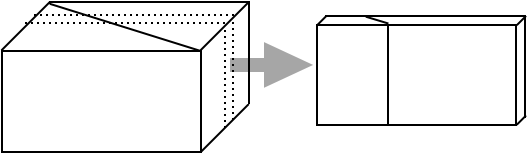
\includegraphics[scale=0.4]{FiguresMaths/CakeHomogeneous3}
        \caption{Cut the two-parts cake in $n$ equal vertical slice.}
        \label{Fig:cakeHomogeneous3}
\end{center}
\end{figure}
Then, cut it into n pieces orthogonally to the icing sides (see Fig.~\ref{Fig:cakeHomogeneous3}). 
This way, each person obtains an equal part composed of two pieces. 
The division is fair because everyone gets exactly the same amount of cake and icing. 
\end{itemize}

In the general cake division problem, the cake is not homogeneous, 
one recipient may like marzipan while another one would rather prefer chocolate or cherries
that are put on the top.
Let us concentrate now on this case.
We detail first the mathematical model of the problem and discuss fairness issues. 


\section{Definitions}

Let us consider a cake to be shared between $n$ \textit{agents}. 
Formally, the cake is represented by the interval $[0,1]$ of real numbers.

A \textit{piece} of the cake is a finite union of disjoint subintervals of $[0,1]$.
We assume that each agent $i$ has her own valuation function (denoted by $v_i$).
This function is a \textit{measure}, $v_i(A)$ represents how much agent $i$ likes piece $A$. 
As the size of the cake has been normalized, the value of the whole cake is equal to $1$
and the value of an empty piece is $0$.
\begin{figure}[htb]
\begin{center}
        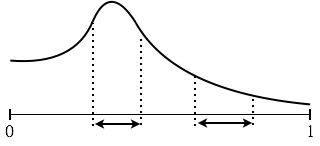
\includegraphics[scale=0.5]{FiguresMaths/cakeMeasure}
        \caption{Mathematical model of a cake and the measure of an agent. 
        Her piece of cake here is the union of the two subintervals 
        (represented by the bold arrows).}
        \label{Fig:cakeMeasure}
\end{center}
\end{figure}

\subsection{Properties}

The assumptions about the valuation of the pieces of cake are:
\begin{itemize}
\item Additivity: $v(A \cup B) = v(A) + v(B)$ for any non-overlapping pieces $A$ and $B$
(pieces are sub-intervals). 
\item 
Continuity: a small increase of a piece leads to a small increase of its value. 
\item The measure of an agent is not known by the others.
\item The resources can be divided into parts of arbitrarily small values.
\end{itemize}

\subsection{Fairness}

The meaning of fair may simply mean a proportional sharing of the resources. 
However, there are more subtil variants:

\begin{itemize}
%\item A cake-cutting protocol is said to be proportionally fair, if each of the $n$ agents can ensure he/she gets an amount of at least $\frac{1}{n}$.
\item The proportional fair division guarantees each recipient (agent) obtains a fair share. 
For instance, if three people divide a cake, each one gets at least a third by her own valuation. 
Formally  for $n$ agents, this corresponds to:

 $v_i(x_i) \geq \frac{1}{n}$ $\forall i$.
\item An envy-free division guarantees that no one will prefer somebody else's piece of cake more than her own piece. 
More formally,  a cake-cutting protocol is called envy-free, if every agent can ensure that she will receive a subjectively largest piece:

 $v_i(x_i) \geq v_i(x_j)$ $\forall i$ and $j$.
\item Equitable division means that every person feels exactly the same happiness, 
i.e. the proportion of the cake an agent receives by her own valuation is the same for everyone. 
This is a difficult aim since the agents need not be truthful if asked their valuations.
Mathematically speaking:  

$v_i(x_i) = v_j(x_j)$ $\forall i$ and $j$.
 \end{itemize}

%Another requirement for all proportionally fair protocols we will discuss, is that agents can guarantee their fair share by answering all questions truthfully.
\bigskip

Observe that for n = 2 agents, we have the following property:

\begin{prop}
For 2 agents, envy-freeness is equivalent to proportional fairness.
\end{prop}

\begin{proof}
Let us prove that proportional fairness implies envy-freeness (the other side of the equivalence is more general since it holds for any $n$, 
and it is proved below in the case $n=3$).

For both agents, proportional fairness means: $v_1(A_1) \geq 1/2$ and $v_2(A_2) \geq 1/2$.
Adding both expressions side by side, we obtain $v_1(A_1)+v_2(A_2) \geq 1$.

Since $v_2(A_1) + v_2(A_2) = 1$, we get 
$v_1(A_1) \geq v_2(A_2)$ and similarly for agent 2. 
\bigskip

The other side of the equivalence is proved as follows: 
Consider the case of $3$ agents who obtained each a piece $A_i$.
The measure of any agent $i$ verifies: $v_i(A_1)+v_i(A_2)+v_i(A_3) = 1$.
Now, as the protocol is envy-free, we also have: $v_1(A_1) \geq v_1(A_2)$ and $v_1(A_1) \geq v_1(A_3)$.
Thus, $3.v_1(A_1) \geq 1$, thus $v_1(A_1) \geq 1/3$ which means that the protocol is proportionally fair. 
\bigskip

But for more than 2 agents, the necessary condition is no longer true.
We detail in section~\ref{sec:movingknives} a counterexample for 3 agents of a proportional protocol which is not envy-free.
\end{proof}


%%%%%%%%%%%%%
\section{Cut-and-choose}

We describe now how to put the division in action with the study of classical protocols.

A fair division protocol lists the actions to be performed by the agents in terms of the visible data and their valuations. 
A valid procedure is one that guarantees a fair division for every player who acts rationally according to their valuation. 
Where an action depends on the valuation of an agent, the procedure describes the strategy a \textit{rational} player would follow. 
She must be consistent,
for instance if a procedure concludes that she cuts the cake in two equal parts, the other player chooses any of both pieces, 
then the first agent cannot claim that the second agent got more...
What the agents should do is:
\begin{itemize}
\item Agree on their criteria for a fair division.
\item Select a valid procedure and strictly follow its rules.
\end{itemize}
%Finally, we assume that the objective of each player is to maximize the minimum amount they might obtain.


\subsection{Two agents}

For two agents, there is a simple solution which is commonly employed.
Many families have been experienced this between their children. 
This is the so-called \textit{cut-and-choose} method, which may be summarize as follows.

One agent, say (1), divides the cake into what she believes are equal halves, and the other one chooses the half she prefers. 

Clearly, the person doing the division has an incentive to divide as fairly as possible. 

It is easy to check that this strategy provides an envy-free division.
However, this solution is not equitable since the non-cutter usually gets more than expected.


\subsection{More than 2}

Let us briefly present a generalization of the previous protocol to more agents
(we examplify it for $n=3$). 

\begin{enumerate}
\item 
Agent (1) cuts the cake into three pieces (which she values equally).
\item 
Agent (2) passes her tour if she thinks at least two of the pieces are $\geq 1/3$ otherwise she labels those two as \textit{bad}. 
\begin{itemize}
\item 
If (2) passed, then agents (3), (2) and (1) each choose a piece in this order and we are done.
\item 
If (2) did not pass, then (3) can also choose between passing and labelling as (2) did. 
If (3) passed, then agents (2), (3) and (1) each choose a piece (in this order) and we are done.
\end{itemize}
\item 
If neither (2) or (3) passed, then (1) has to take one of the pieces labelled as bad by both (2) and (3).

Then, the final solution is obtained by playing cut-and-choose between (2) and (3).
\end{enumerate}


%%%%%%%%%%%%
\section{Moving knives}
\label{sec:movingknives}

\subsection{The basic strategy with two agents}

The moving-knife procedure that is described below for $n$ agents gives an \textbf{exact} division for two agents\footnote{Dubins and Spanier. 
\textit{How to Cut a Cake Fairly.}  American Mathematical Monthly, 68(1):1–17, 1961.}. 

First, let us assume that there exists an external referee who is managing the knife. 

%There exists a moment when the division is fair.

(i) The referee moves a knife slowly across the cake, from left to right. 
Any agent may shout \textbf{stop} at any moment. Whoever does so receives the piece that is at the left of the knife.

(ii) When a piece has been cut off, we continue with the remaining agents, until just one agent is left (who takes the rest).
\bigskip 

Now, let us study what happens if we remove the external referee. 
For two agents, a way to do this is as follows:

\begin{enumerate}
\item 
Agent (1) places two knives over the cake such that one knife is at the left side of the cake and one is further right; 
half of the cake lies between the knives. 
She then moves the knives right, always ensuring there is half the cake – by his valuation – between the knives. 
If she reaches the right side of the cake, the leftmost knife must be where the rightmost knife started off. 
\item Agent (2) stops when he/she thinks there is half the cake between the knives. 
%{\Denis Give the argument why there is always a point at which this happens?}
\end{enumerate}
\bigskip

This protocol is proportionally fair, but it is not envy-free. 
Proving that this last condition does not hold is easy by looking at the following counter-example
of three agents denoted in the figures by (1), (2) and (3).
(3) is jealous about the piece obtained by (2). 
\begin{figure}[htb]
\begin{center}
        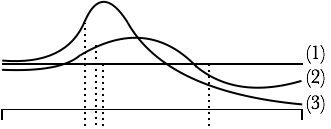
\includegraphics[scale=0.6]{FiguresMaths/CakeEnvyFree1}
        \caption{Example of the distribution of the measures for 3 agents.
        The dotted vertical lines show 1/3 of the measure for each agent.}
        \label{Fig:cakeEnvyFree1}
\end{center}
\end{figure}
\begin{figure}[htb]
\begin{center}
        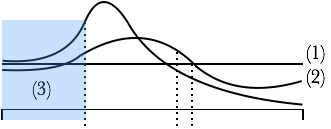
\includegraphics[scale=0.6]{FiguresMaths/CakeEnvyFree2}
        \caption{Agent (3) stops first and get exactly 1/3 of her measure (shaded area).
        The remaining agents (1) and (2) share the rest of the cake. }
        \label{Fig:cakeEnvyFree2}
\end{center}
\end{figure}
\begin{figure}[htb]
\begin{center}
        \includegraphics[scale=0.6]{FiguresMaths/CakeEnvyFree3}
        \caption{(2) stops when she gets 1/3 of her measure (shaded area) and finally, (1) gets the rest of the cake.}
        \label{Fig:cakeEnvyFree3}
\end{center}
\end{figure}


\subsection{Extension to 3 agents}

The moving knife strategy can be adapted to guarantee envy-freeness for 3 agents\footnote{W. Stromquist.
\textit{How to Cut a Cake Fairly.} American Mathematical Monthly, 87(8), 1980.}
with a protocol using $4$ knives, one for an external referee and one for each agent.

\begin{enumerate}
\item
A referee slowly moves a knife across the cake, from left to right.
\item
At the same time, each agent is moving her own knife so that she would cut the righthand piece in half 
(with regard to their own valuations).
\item
The first agent to shout stop receives the piece to the left of the referee’s knife. 
The righthand part is cut by the middle of the three agent knives. 
If neither of the other two agents hold the middle knife, they each obtain the piece at which their knife is pointing. 
If one of them holds the middle knife, then the other one gets the piece at which her knife is pointing.
\end{enumerate}
\bigskip

It is rather simple to prove the proportional fairness.
A nice exercise is to show that this sophisticated protocol is envy-free. The proofs are left to the readers. 


\subsection{Evaluation of the complexity}

Coming back to the basic moving knife strategy, each agent has to evaluate the measure as the knife moves over (for all the real numbers in the interval). 
For each continuous position, the agent has to evaluate the piece at the left of the knife.

Again, the mathematics helps us to evaluate the protocols by providing a \textit{model}.
Each protocol should be implementable in terms of two types of queries for agent $i$:
 \begin{itemize}
 \item $cut_i(\alpha,x) \rightarrow y$ -- agent $i$ cuts the part of value $\alpha$ in the interval from $x$ to $y$. 
 \item $v_i(x,y) \rightarrow \alpha$ -- is the evaluation of the measure of agent $i$  between $x$ and $y$.
 \end{itemize}
 
According to the number of queries, we are able to compare the complexity of protocols.
For instance, we can simulate the continuous moving knife protocol as follows:

\begin{enumerate}
\item
Ask each agent to mark the cake where she would shout stop.
Then cut the cake at the leftmost mark and give the resulting piece to the agent who made that mark.
\item
When a piece has been cut off, we continue with the remaining agents, until just one agent is left (who takes the rest).
\end{enumerate}

At each round, each participating agent makes one mark. 
The number of participating agents goes down from $n$ to $2$ for a total cost of $\Delta_n -1$, 
where $\Delta_n$ denotes the $n$th triangular number. 


%%%%%%%%%%%%%%%%

\ignore{
\bigskip

Even and Paz introduced in 1984 the following divide-and-conquer protocol,
which improves the complexity:

(1) Each agent puts a mark on the cake at half of his/her own measure. 

(2) Cut the cake at the $\lfloor \frac{n}{2} \rfloor$-th mark (counting from the left). 
Associate the agents who made the leftmost $\lfloor \frac{n}{2} \rfloor$ marks with the 
lefthand part, and the remaining agents with the righthand part. 

(3) Repeat for each group in all the intervals, until only one agent is left.

It is easy to show that this division is also proportionally fair.

The complexity is $log_2(n)$ steps involving each $n$ operations. 
\bigskip

Note that there are more sophisticated protocols...
}


\section{A more sophisticated method}

Let us now present an envy-free solution for $3$ agents.

(1) Agent 1 cuts the cake in three pieces (she considers equal).

(2) Agent 2 either “passes” (if she thinks at least two pieces are tied for largest) or cuts one piece (to get two tied for largest pieces).
If she passed, then let agents 3, 2 pick in this order, and then, 1.

(3) If agent 2 did cut, then let 3, 2 pick (in this order), but require 2 to take the cutted piece (unless 3 did) and then, 1. 
Keep the cuts unallocated for now (notice that the partial allocation is envy-free).

(4) Now divide the cuts. 
Whoever of 2 and 3 received the uncutted piece does the cutting. 
Let agents choose in this order: non-cutter, 1, cutter.

{\Denis Add a figure here}



\ignore{
\begin{thebibliography}{1}

\bibitem{Barbanel}
J. Barbanel and S. Brams.
\newblock {C}ake division with minimal cuts: envy-free procedures for 3 persons, 4 persons and beyond.
\newblock NY university, 2004.

%\bibitem{Dublins}
%L. Dubins and E.H. Spanier. 
%\newblock How to Cut a Cake Fairly. 
%\newblock American Mathematical Monthly, 68(1):1–17, 1961.

\bibitem{Endriss}
U. Endriss. 
\newblock Lecture Notes on Fair Division. 
\newblock ILLC, University of Amsterdam, 2009.

\bibitem{Robertson}
J. Robertson and W. Webb.
\newblock {C}ake-{C}utting Algorithms: Be Fair If You Can.
\newblock Natick, Massachusetts: A. Peters, 1998.

%\bibitem{Stromquist}
%W. Stromquist.
%\newblock How to Cut a Cake Fairly. 
%\newblock American Mathematical Monthly, 87(8):640–644, 1980.

 
\end{thebibliography}{}
}
